\documentclass[xelatex,11pt, xcolor=dvipsnames]{beamer}
\usepackage{pgfpages}
\usepackage{fontspec}
\usepackage{polyglossia}
\PolyglossiaSetup{french}{indentfirst=false}
\usepackage[french=guillemets]{csquotes}
\usepackage{xpatch}
\usepackage{diagbox}

\setmainlanguage{french}
\xapptocmd\ttfamily{\XeTeXinterchartokenstate=0 }{}{}
\newcommand{\nospace}[1]{\texttt{#1}}

\usepackage{algorithm}
\usepackage[noend]{algpseudocode}
    \newcounter{lastenum}
    \newcommand{\mtpause}{\setcounter{lastenum}{\value{enumi}}}
    \newcommand{\mtresume}{\setcounter{enumi}{\value{lastenum}}}
\resetcounteronoverlays{lastenum}

\usepackage[backend=biber]{biblatex}
\addbibresource{Modele.bib} 
\bibliography{Modele}
\setbeamertemplate{bibliography item}[triangle]

\usepackage{multirow} % row fusion
\usepackage{array} % column fusion
\usepackage{xfrac} % small fractions
\usepackage{adjustbox}
\usepackage{listings}
\usepackage{dirtree}

\usetheme{Warsaw}
\usecolortheme{wolverine}

\setbeamertemplate{frametitle}{
	\nointerlineskip  
	\begin{beamercolorbox}[wd=\paperwidth,ht=2.75ex,dp=1.375ex]{frametitle}
		\hspace*{2ex}\insertframetitle \hfill {
			\small\insertframenumber/\inserttotalframenumber
		} \hspace*{1ex}%
    	\end{beamercolorbox}
}

 \titlegraphic{\vspace{-1cm}
      \includegraphics[width=2.5cm]{images/paris8_1}\hspace*{4.75cm}~%
      \hfill
      \includegraphics[width=2.5cm]{images/logo}
}

\beamertemplatenavigationsymbolsempty
\setbeamertemplate{blocks}[rounded][shadow=true]
\setbeamerfont{page number in head/foot}{size=\large}

% Parties conditionnelles
\usepackage{etoolbox} % pour toggle
\newtoggle{bandeaularge}
\newtoggle{MSsanspuces}


% Ici on choisit si on veut un bandeau en largeur (pas de sous section) ou normal
\toggletrue{bandeaularge}% commenter pour passer au bandeau normal

% Bandeau en largeur
\iftoggle{bandeaularge}
{%
  \setbeamertemplate{headline}{%
    \hbox{%
      \begin{beamercolorbox}[wd=\paperwidth, ht=2.8ex, dp=1ex]{section in head/foot}%
      \insertsectionnavigationhorizontal{\paperwidth}{}{}%
      \end{beamercolorbox}%
  }%
}%
\setbeamertemplate{section in head/foot}%
{\colorbox{yellow!90!orange}{\insertsectionhead}}%
% Essai pour élargir le titre courant mais pas terrible
%\setbeamertemplate{section in head/foot}{\colorbox{yellow!90!orange}{\parbox{10em}{\centering\color{black}\insertsectionhead\par}}}
}%{}

\iftoggle{MSsanspuces}{%
\setbeamertemplate{itemize items}[bullet]}{}

\subtitle{Cours Ingénierie des langues\\\textbf{Projet, 1ère phase}}
\institute{\normalsize Université Paris 8, LIASD\\
Licence d'informatique}

% Les utilisateurs sous Windows qui ne voient pas de puces doivent décommenter la ligne suivante
%\toggletrue{MSsanspuces}

% Ici on choisit si on veut seulement les diapos ou le texte à lire sur son écran

\setbeameroption{hide notes} % Only slides
%\setbeameroption{show only notes} % Only notes
%\setbeameroption{show notes on second screen=right} % Both

% Ici on indique son titre et son nom

\title{Projet Errol - Catégorisation des mails en HAM et SPAM}
\author[\textsc{M. Goehry}]{\textsc{Martial Goehry}}


\begin{document}
{ \setbeamertemplate{headline}{}
  \setbeamertemplate{footline}{}
  \begin{frame}
  \titlepage
  \end{frame}

\note{
}
}

\begin{frame}{Plan}
  \tableofcontents[sectionstyle=show/show, hidesubsections]
\note{
}  
\end{frame}

\begin{frame}{Objectif}
	\begin{block}{}
		L'objectif est d'extraire des données d'e-mails pour déterminer s'ils sont des courriers légitimes ou de sollicitations indésirées.
	\end{block}
	\begin{itemize}
		\item langue concernée : Anglais
		\item type de corpus : corpus monolingue écrit
		\item type de données : e-mail
	\end{itemize}
\end{frame}


\section{Général}

\begin{frame}{Présentation de l'insfrastructure}
	Les traitements sont basés sur un ensemble de d'instruction écrites en Python.\\
	L'infrastructure de données utilise 1 base NoSQL (mongoDB) et 2 bases SQL (Postgres et SQLite).\\
	Les moteurs et services sont conteneurisés pour limiter l'impact sur la machine hôtes.\\
	L'initialisation des schémas des bases de données est gérée directement par le programme Python.\\
\end{frame}

\begin{frame}
	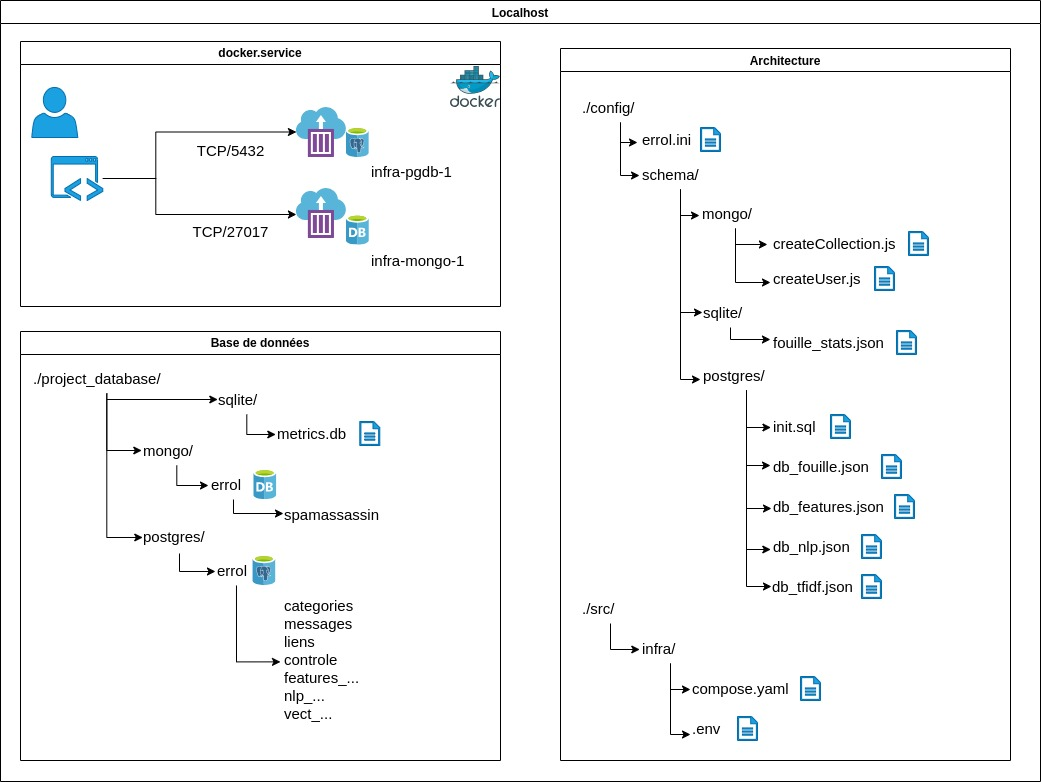
\includegraphics[width=\linewidth]{img/SchemaDocker}
\end{frame}

\begin{frame}{Déroulé}
	L'éxécution des traitements se déroule en plusieurs phases:
	\begin{itemize}
		\item Importation des données et prétraitement (fouille.py)
		\item Recherche de caractéristiques (features.py)
		\item Traitement du langage naturel (nlp.py)
		\item Vectorisation (vecteurs.py)
	\end{itemize}

	\begin{block}{Manquant}
		La partie sur l'utilisation des vecteurs dans un modèle d'apprentissage n'est pas traitée
	\end{block}
\end{frame}

\begin{frame}
	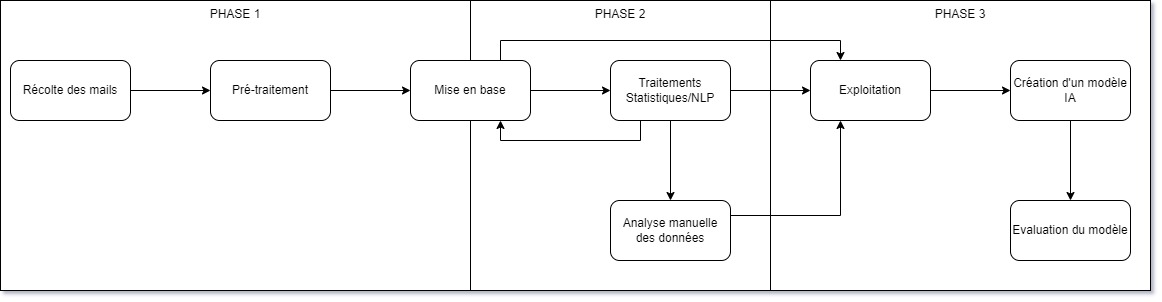
\includegraphics[width=\linewidth]{img/SchemaGeneral}
\end{frame}

\section{Fouille}
\begin{frame}{Récupération des mails}
	Faute de sources, il n'a pas été possible de mettre en place une automatisation pour la récupération des mails.
	Il a été nécessaire de les récupérer manuellement dans d'autres projets du même type
	\begin{block}{Alternative}
		Une autre possibilité est de créer un site web dans lequel les utilisateurs auraient pu ajouter des nouveaux documents.
		Il aurait fallu prendre en compte la mise en place de cette architecture et les règlementations RGPD\@.
	\end{block}
\end{frame}

\begin{frame}{Corpus}
	\begin{block}{Dataset de mail du projet SpamAssassin}
		\begin{itemize}
			\item Anglais
			\item \url{https://spamassassin.apache.org/old/publiccorpus/}
			\item consulté le 27/01/2022
			\item environ 6000 fichiers email déjà trier en ham et spam
		\end{itemize}
	\end{block}
	
	\begin{block}{Dataset de mail de la compagnie Enron}
		\begin{itemize}
			\item Anglais
			\item \url{https://www.kaggle.com/wcukierski/enron-email-dataset}
			\item consulté le 27/01/2022
			\item fichier CSV avec 33 millions de lignes (un mail par ligne) non trié
			\item Non utilisé ici
		\end{itemize}
	\end{block}
\end{frame}


\begin{frame}{Etapes}
	Afin d'accélérer cette phase, chaque mail est traité dans un processus à par grace au \emph{multiprocessing.Pool()}.
	\begin{block}{Importation}
		Les mails sont chargé en mémoire depuis les fichiers en utilisant la fonction \emph{email.message\_from\_binary\_file()}
	\end{block}

	\begin{block}{Extraction}
		Un mail peut être multipart.
		On récupère récursivement uniquement les types text/plain, text/html, text/enriched.
		Les Headers et les autres types de MIME sont ignorés (audio, video, image...)
	\end{block}
\end{frame}

\begin{frame}{Etapes: Nettoyage}
	Cette étape permettre de nettoyer le texte de certains éléments non souhaités :
	\begin{enumerate}
		\item Suppression des balises html avec le module \emph{BeautifulSoup} (bs4)
		\item Suppression des balises enriched text avec le module \emph{re}
		\item Suppression des réponses avec le module \emph{re}
		\item Substitutions des adresses mail, url et numéro de téléphone avec le module \emph{re}
		\item Substitutions des prix et des nombres avec le module \emph{re}
		\item Suppression des ponctuations superflues avec le module \emph{re}
	\end{enumerate}
\end{frame}

\begin{frame}[fragile]{Expressions régulières du nettoyage}
	\begin{itemize}
		\item Capture des balises enriched text: \verb'<.*>'
		\item Capture des réponses: \verb'^>.*$'
		\item Capture mail: \verb'[a-zA-Z0-9_.+-]+@[a-zA-Z0-9-]+\\.[a-zA-Z0-9-.]+'
		\item Capture url: \verb'(http|ftp|https)?:\/\/([\w\-_]+(?:(?:\.[\w\-_]+)+))'
							\verb'([\w\-\.,@?^=%&:/~\+#]*[\w\-\@?^=%&/~\+#])?'
		\item Capture téléphone1: \verb'\\(\\d{3}\\)\\d+-\\d+'
		\item Capture téléphone2: \verb'\\+\\d+([ .-]?\\d)+'
		\item Capture prix1: \verb'[$€£]( )?\\d+([.,]\\d+)? '
		\item Capture prix2: \verb' \\d+([.,]\\d+)?( )?[$€£]'
		\item Capture nombre: \verb'\\d+'
	\end{itemize}
\end{frame}

\begin{frame}{Fouille - difficultés}
	\begin{block}{Encodage}
		Certains encodages ne sont pas pris en charge par le module \emph{email}.
		J'ai dû me limiter aux encodages suivants : ascii, Windows-1252, ISO-8859-1, utf-8.\\
		J'utilise le module \emph{chardet} pour faire la détection de l'encodage
	\end{block}

	\begin{block}{Multiple charset}
		Les messages mails peuvent avoir plusieurs charset à l'intérieur du payload (\emph{get\_content\_charset}).
		Les charset suivant m'ont posé des problèmes lors du traitement, j'ai écarté : unknown-8bit, default, default\_charset, gb2312\_charset, chinesebig5, big5.\\
		Écarter ces charset permet d'enlever les messages écrits en turc, chinois ou japonais.
	\end{block}
\end{frame}

\begin{frame}{Fouille - difficultés}
	\begin{block}{Langues}
		Le corpus contenant des mails dans d'autres langues.
		J'ai fait appel au module langdetect pour exclure les mails qui ne sont pas majoritairement en anglais.
	\end{block}
\end{frame}


\begin{frame}{Exemple de nettoyage texte brut}
	\begin{block}{Brut}
Message dedicated to be a sample to show how the process is clearing the text.

Begin reply :
> He once said
>>> that it would be great
End of reply.
Substitutions :
spamassassin-talk@example.sourceforge.net
https://www.inphonic.com/r.asp?r=sourceforge1\&refcode1=vs33
hello.foo.bar
between \$ 25 and 25,21 \$

A number is : 2588,8 588
Phone type a : (359)1234-1000
Phone type b : +34 936 00 23 23
Ponctuation : ----\#\# ..
	\end{block}
		
	\begin{block}{Nettoyé}
message dedicated to be a sample to show how the process is clearing the text. begin reply end of reply. substitutions MAIL URL URL between PRIX and PRIX a number is NOMBRE , NOMBRE NOMBRE phone type a TEL phone type b TEL ponctuation . 
	\end{block}

\end{frame}

\begin{frame}{Nettoyage enriched text}

	\begin{block}{Brut}
	<smaller>I'd like to swap with someone also using Simple DNS to take
advantage of the trusted zone file transfer option.</smaller>
	\end{block}
	
	\begin{block}{Nettoyé}
	I'd like to swap with someone also using Simple DNS to take
advantage of the trusted zone file transfer option.
	\end{block}
	
\end{frame}

\begin{frame}[fragile]{Nettoyage HTML brut}
\small
\begin{verbatim}
<!DOCTYPE html PUBLIC "-//W3C//DTD HTML 4.01 Transitional//EN">
<html>
<head>
  <title>Foobar</title>
</head>
<body>
I actually thought of this kind of active chat at AOL 
bringing up ads based on what was being discussed and 
other features
  <pre wrap="">On 10/2/02 12:00 PM, "Mr. FoRK" 
  <a class="moz-txt-link-rfc2396E"href="mailto:fork_
  list@hotmail.com">&lt;fork_list@hotmail.com&gt;</a> 
  wrote: Hello There, General Kenobi !?
<br>
</body>
</html>
\end{verbatim}
\normalsize
	
\end{frame}

\begin{frame}[fragile]{Nettoyage HTML nettoyé}
\small
\begin{verbatim}
Foobar


I actually thought of this kind of active chat at AOL 
bringing up ads based on what was being discussed and 
other features
  On 10/2/02 12:00 PM, "Mr. FoRK" 
   
  wrote: Hello There, General Kenobi !?
\end{verbatim}
\normalsize
\end{frame}

\begin{frame}
	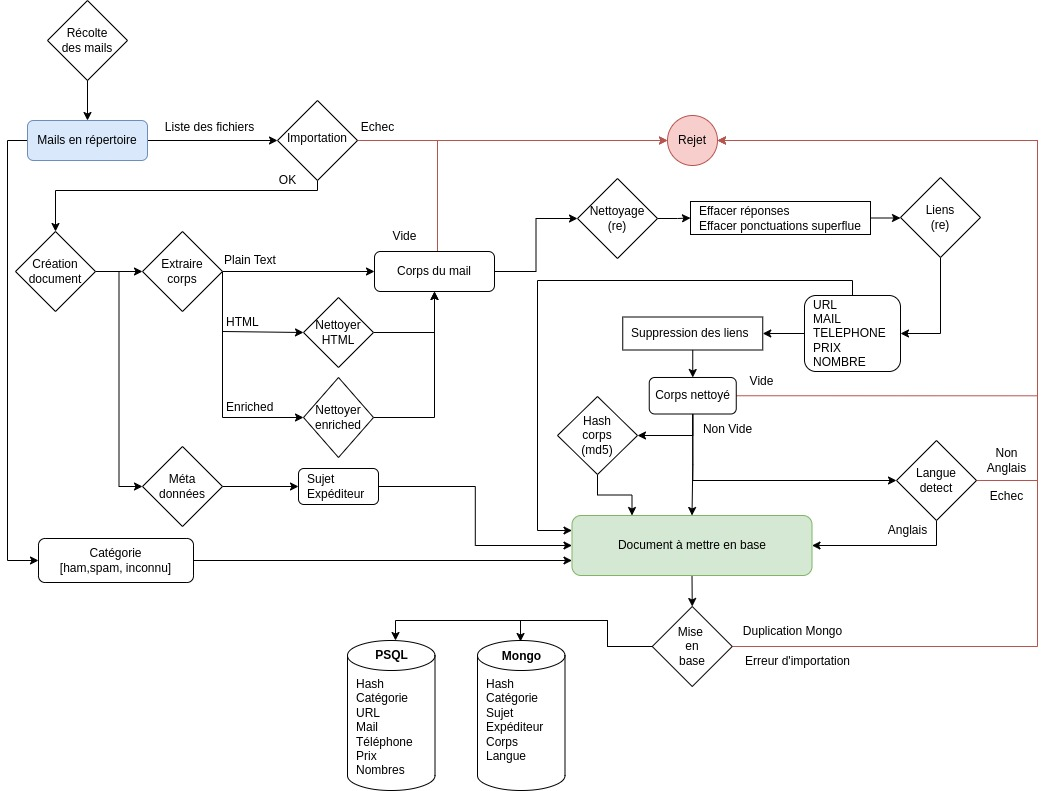
\includegraphics[width=\linewidth]{img/SchemaPhase1}
\end{frame}

\begin{frame}
	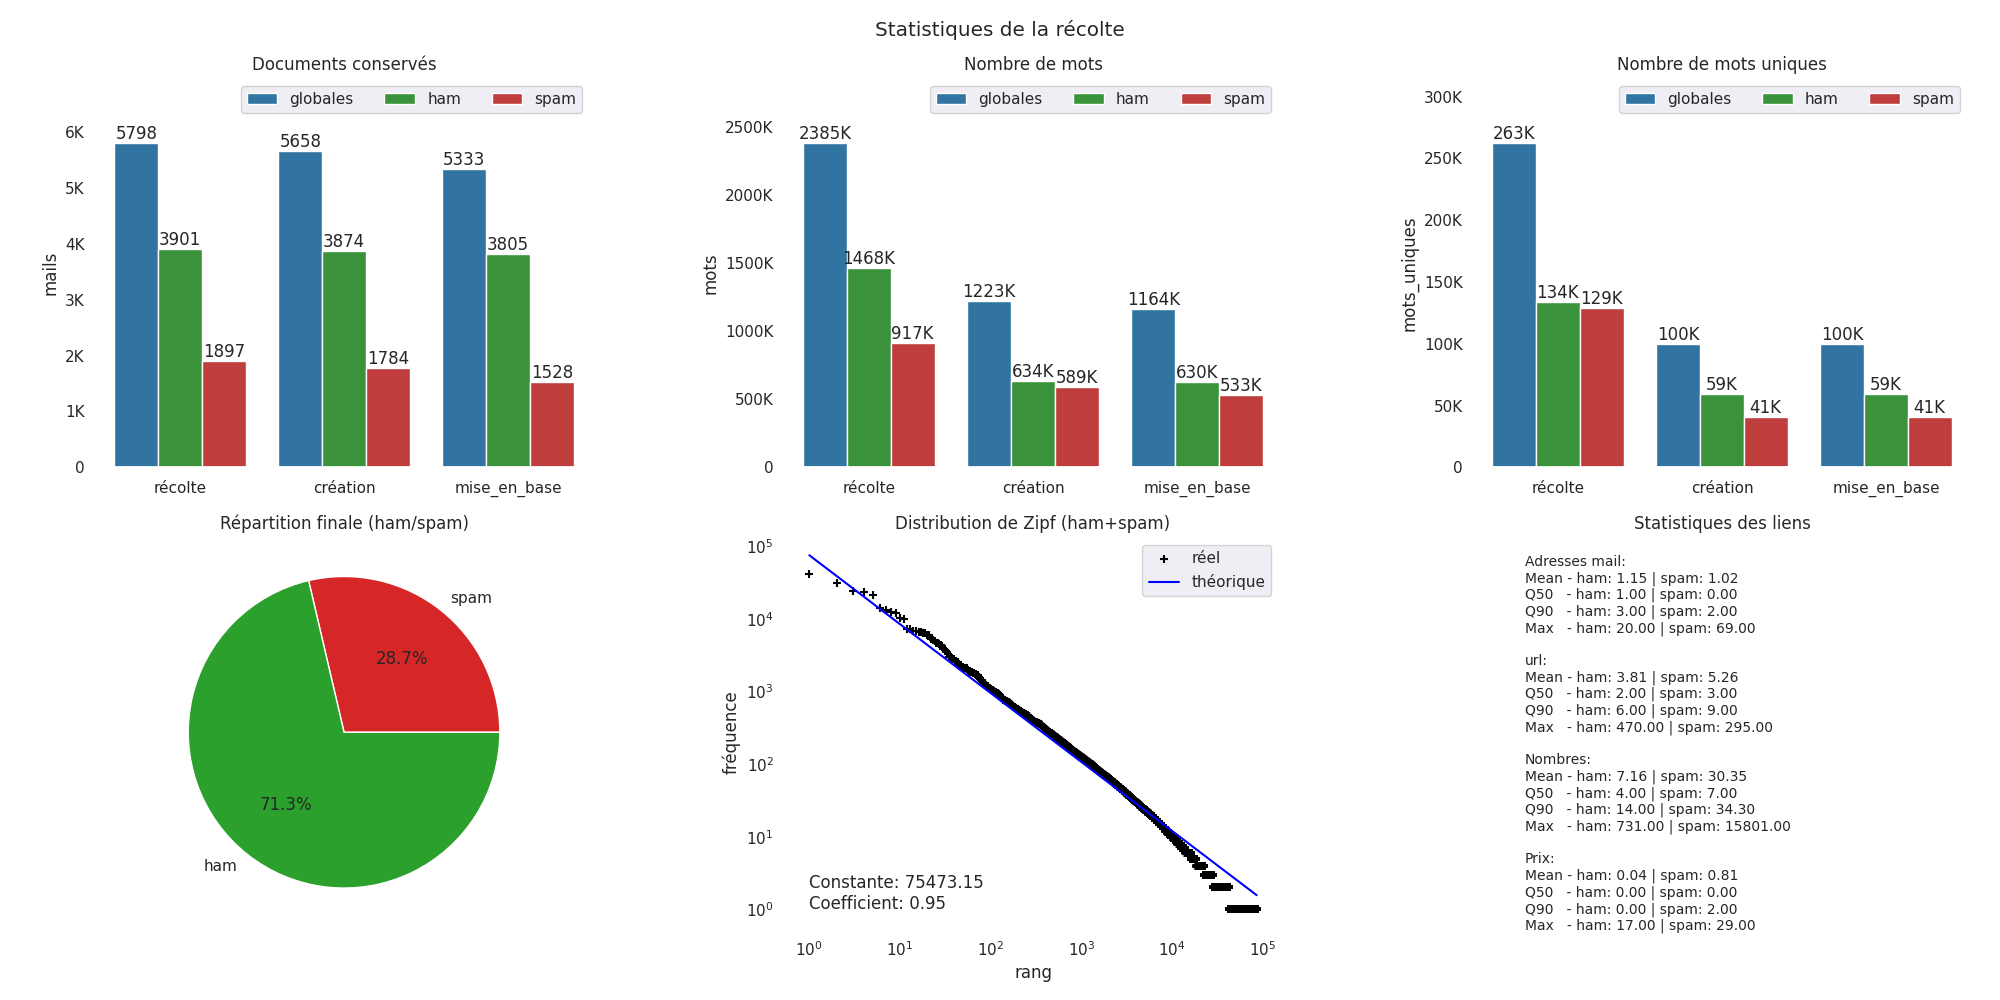
\includegraphics[width=\linewidth]{img/fouilleStats}
	Les substitutions des adresses mails, des liens et des nombres, n'est pas très concluante.
\end{frame}


\section{Caractéristiques}
\begin{frame}{Recherche de caractéristiques}
	Cette étape va se concentrer sur la forme plutôt que sur le fond.
	L'idée est de comprendre si certains éléments non textuels sont plus présent dans un type que dans un autre
	\begin{block}{Eléments recherchés}
		\begin{itemize}
			\item Nombre de chars en majuscule et minuscule
			\item Nombre de mots en majuscule et capitalisé
			\item Nombre de ponctuations simple (point, virgule, exclamation, interrogation)
			\item Nombre d'espaces (espaces, tabulation, ligne vide)
			\item Nombre de lignes
			\item Données de la distribution de Zipf (constante, coefficient)
			\item Données de la rechercher d'Hapax (nombre, ratio dans le texte et dans la liste des mots uniques)
		\end{itemize}
	\end{block}
\end{frame}

\begin{frame}{Exécution}
	Plusieurs fonctions de comptage sont executées itérativement sur chaque message.
	Toujours dans un souci de performance, le module multiprocessing est utilisé.\\

	Le schéma si dessous montre les étapes de cette phase.
	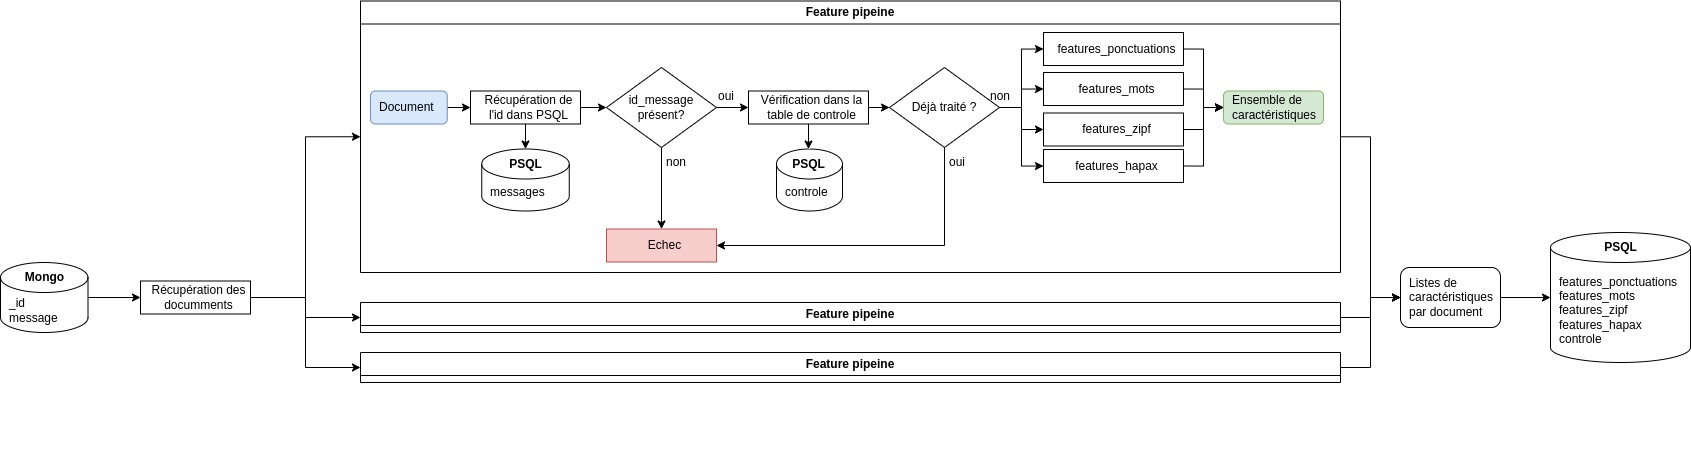
\includegraphics[width=\linewidth]{img/features}
	\begin{block}{Methodes python utilisée}
		\begin{itemize}
			\item str.count(...)
			\item len(re.findall(...))
		\end{itemize}
	\end{block}
\end{frame}

\begin{frame}{Résultats}
	Sans représenter les détails du rapport, on peut lister les éléments suivants:
	\begin{itemize}
		\item Les spams utilisent plus de mots et de mots uniques
		\item Les mots complètement en majuscules sont très peu utilisés
		\item L'utilisation des ponctuations et des espaces est plus prononcé dans les spam
	\end{itemize}
	\begin{block}{Caractéristiques retenues}
		\begin{itemize}
			\item ratio-mots-uniques
			\item nombre hapax
			\item char-majuscule
			\item espaces
		\end{itemize}
	\end{block}
\end{frame}

\begin{frame}{Covariance des caractéristiques}
	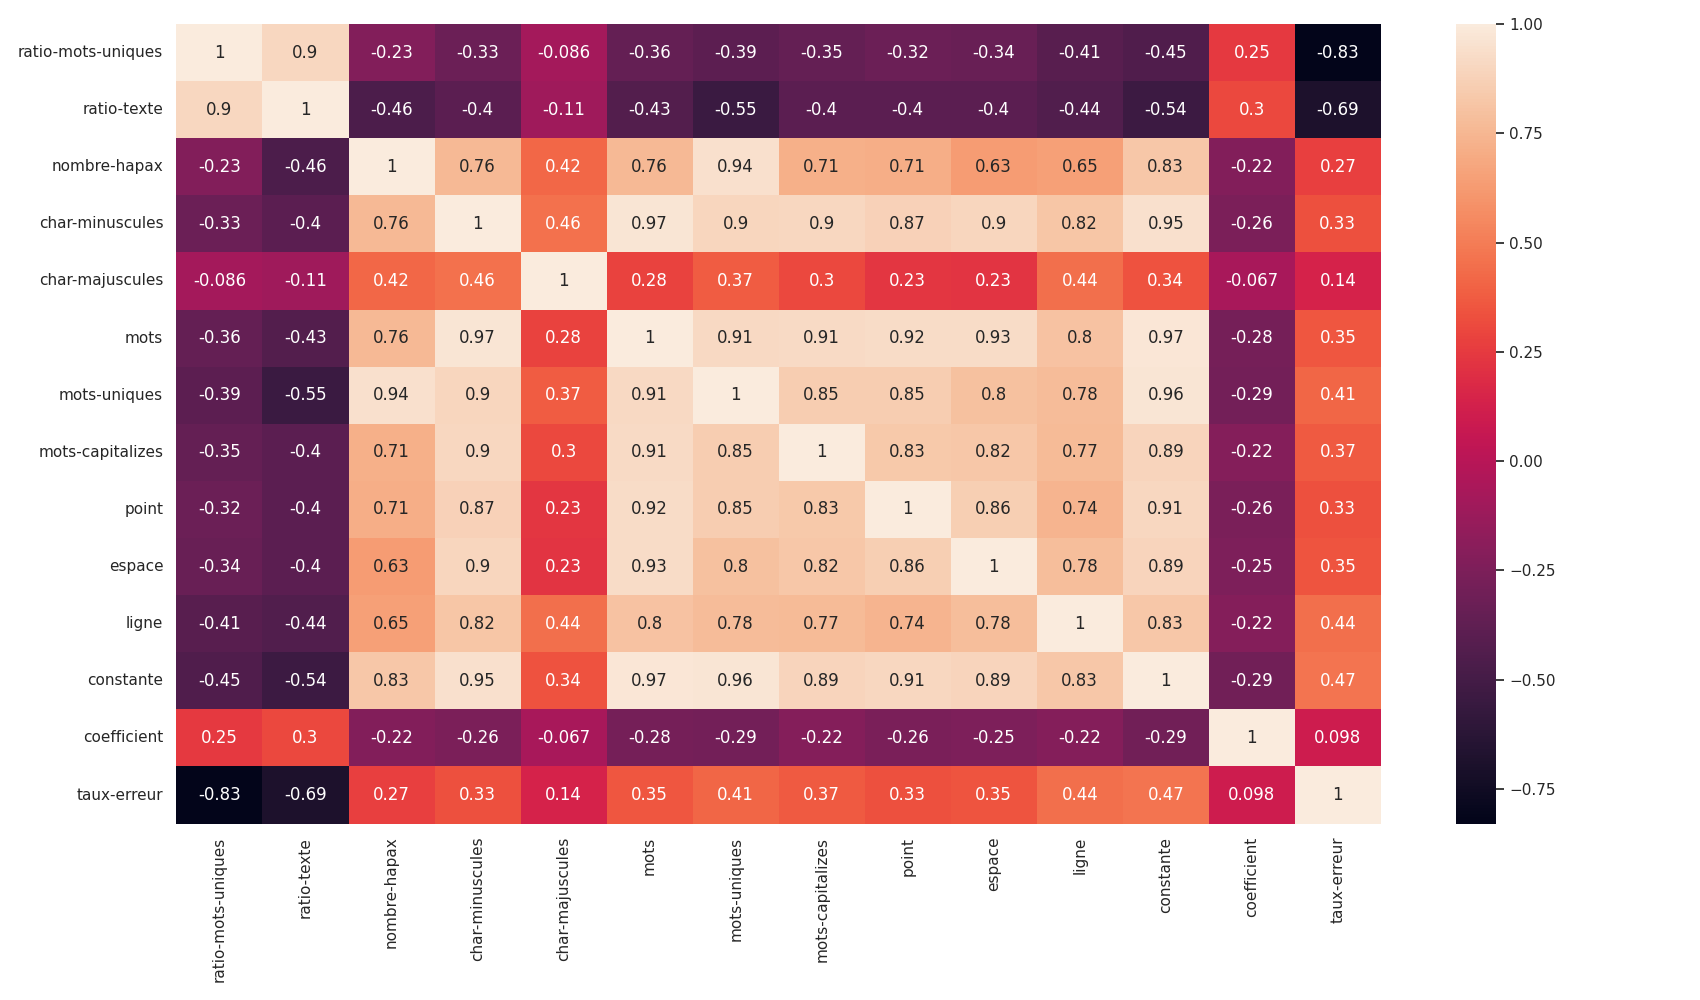
\includegraphics[width=\linewidth]{img/features_corr}
\end{frame}

\section{Traitement du langage}
\begin{frame}{Traitement du langage}
	La technique choisie est la lemmatisation en utilisant le modèle neuronal de StandfordNLP (Stanza).
	\begin{block}{Etapes de la pipeline Stanza}
		\begin{enumerate}
			\item Tokenisation
			\item Multi-Word Token Expansion
			\item Part Of Speech Tagging
			\item Lemmatisation
		\end{enumerate}
	\end{block}
	Le comptage des mots est effectué par une fonction annexe (\emph{zipf.freq\_mot()})
	L'utilisation du multiprocessing n'est pas possible ici du fait de l'utilisation de CUDA et la carte graphique.
	
\end{frame}

\begin{frame}{Traitement du langage}
	Schéma d'éxecution:
	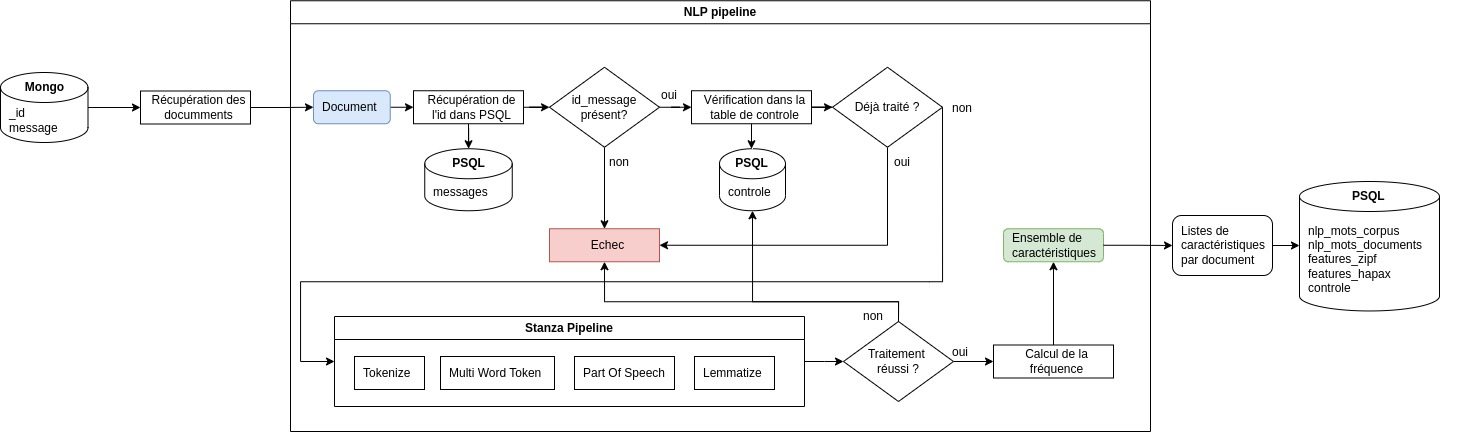
\includegraphics[width=\linewidth]{img/nlp}
	Tableau des résultats:
	\begin{table}[H]
            \centering
            \begin{tabular}{l|rr}
                catégorie & mots & mots uniques \\
                global & 658524 & 39947 \\
                \hline
                ham & 355595 & 27787 \\
                \hline
                spam & 302929 & 19852 \\
            \end{tabular}
        \end{table}
\end{frame}

\section{Vectorisation}
\begin{frame}{Vectorisation}
	En se basant sur une liste des mots les plus fréquents (ici 2940), il a été possible de transformer ces 5333 textes en données numériques.
	La méthode de vectorisation est celle du Term Frequency-Inverse Document Frequency (TFIDF).
	\begin{block}{Echantillons de mots du vecteur}
		list, get, use, email, one, make, free, time, person, send, new, information, would, work,
 		say, receive, good, like, write, message, go, business, mailing, address, please, click,
 		order, money, year, want, report, name, need, find, know, also, see, take, company, day,
 		e-mail, remove, group, file, site, change, system, mail, program, look,...
	\end{block}
	Les mots sans connotations de sens ont été retiré du vecteur.
\end{frame}


\begin{frame}{Schéma de la vectorisation}
	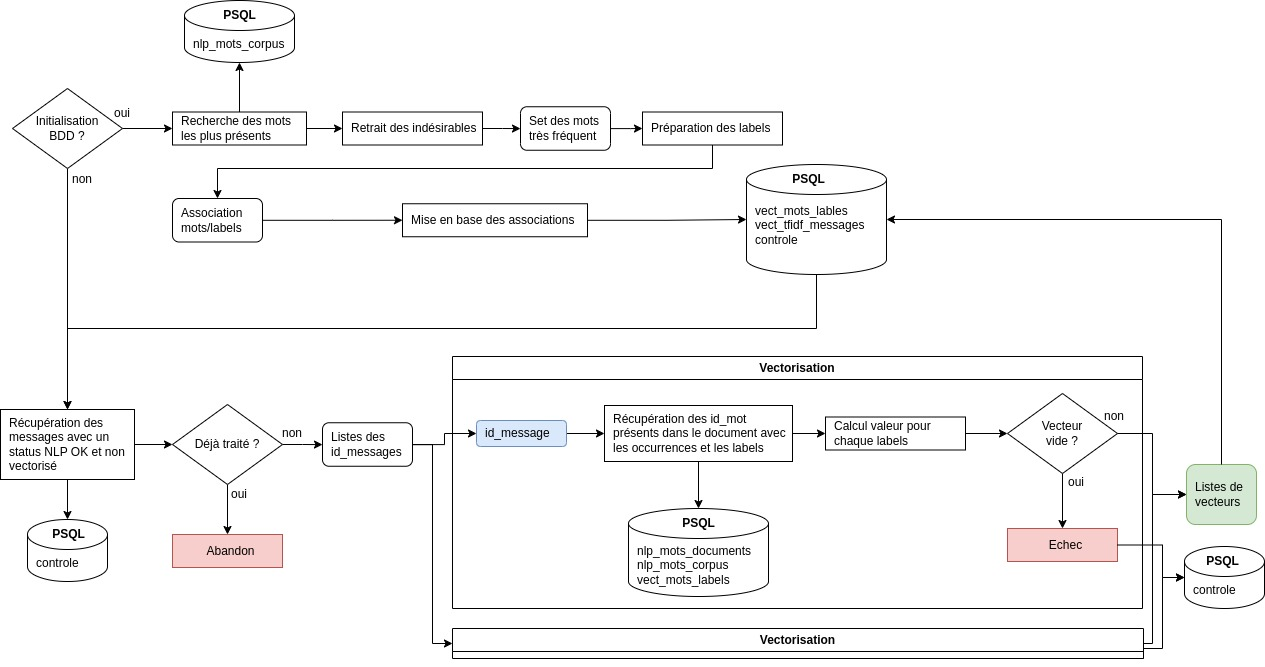
\includegraphics[width=\linewidth]{img/tfidf}.
	Il a été à nouveau possible d'utiliser le multiprocessing sur cette action.
\end{frame}

\begin{frame}{Résultats}
	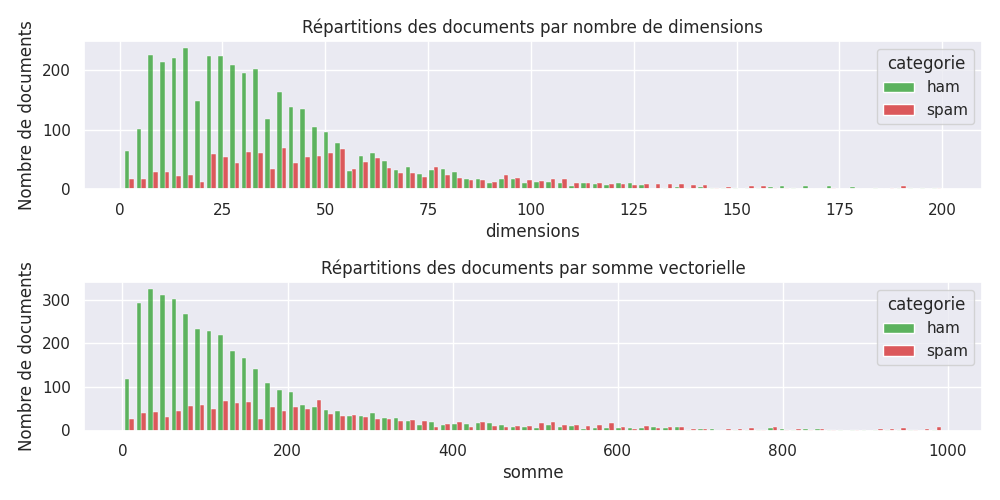
\includegraphics[width=\linewidth]{img/vectdash}
\end{frame}

\begin{frame}{Résultats}
	\centering
	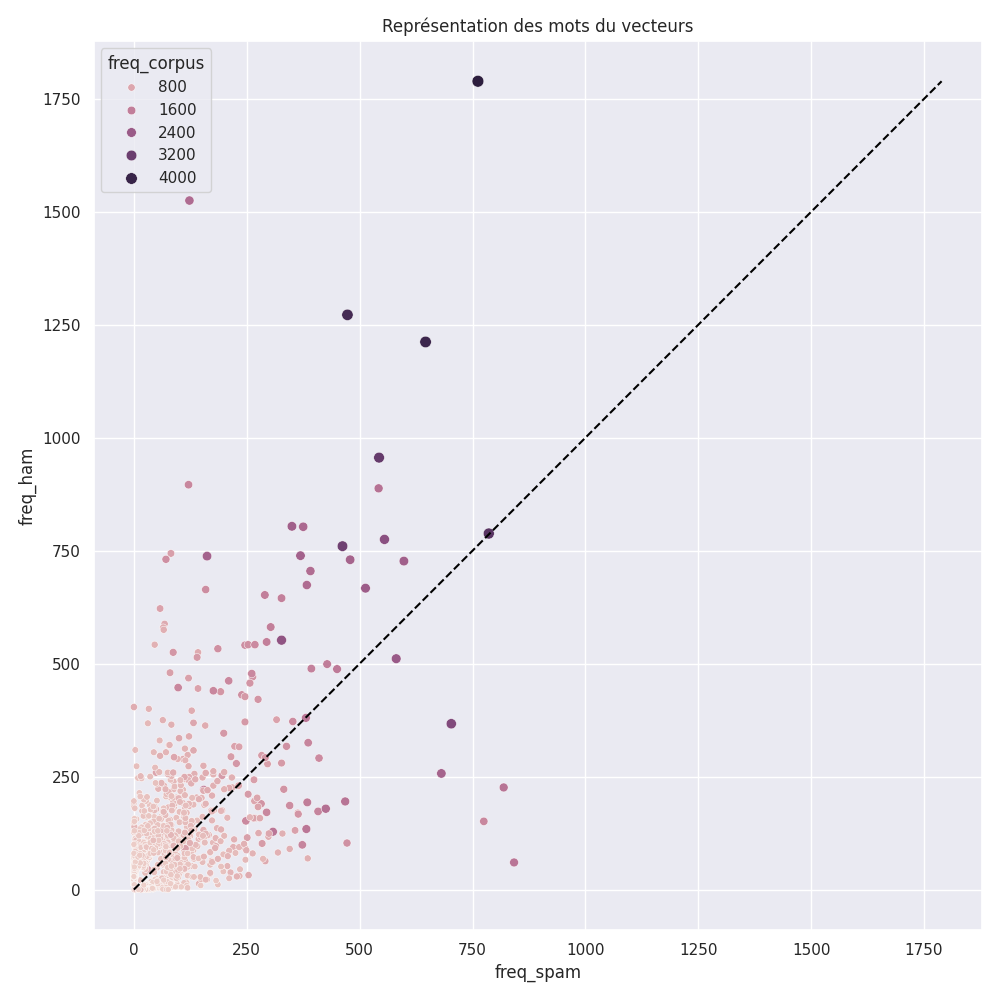
\includegraphics[scale=0.3]{img/vectmots}
\end{frame}

\section{Conclusion}
\begin{frame}{Conclusion}
	Il a été possible d'effectuer tout un ensemble de traitement pour convertir des éléments textuels en données numériques.
	Ces opérations successives ont considérablement réduit le volume de données à traiter pour les modèles d'apprentissage.
	\begin{table}[H]
	\begin{tabular}{l|rrr]}
        Phase/Etape & documents & mots & mots uniques\\
        \hline
		Récolte & 5798 & 2385120 & 262614\\
		Transformation & 5658 & 1222793 & 99772\\
		Sauvegarde & 5333 & 1163550 & 99772\\
		Traitement du langage & 5333 & 658524 & 39947\\
		Vectorisation & 5333 & 453068 & 2942\\
	\end{tabular}
	\end{table}
\end{frame}

\begin{frame}{Et ensuite}
	\begin{block}{Modélisation}
		Les étapes de modélisation et d'apprentissage ne sont pas présentes ici.
		Lors de la version précédente du projet, j'avais obtenu des résultats encourageant avec Random Tree Forest ou Support Vector Machine.
	\end{block}

	\begin{block}{Amélioration}
		L'analyse actuelle n'est pas très poussée pour la recherche de données abérrantes qui pourrait corrompre les modèles futurs.
	\end{block}
\end{frame}

% éléments hors section
\appendix

%  \begin{frame}{Références}%[allowframebreaks]
%  \renewcommand*{\bibfont}{\footnotesize}
%  \nocite{*}
%  \printbibliography[heading=none]
%  \begin{itemize}
%  	\item Documentation du paquet email de python, [en ligne], \url{https://docs.python.org/fr/3/library/email.html} (27/01/2022)
%  	\item Documentation du paquet regex de python, [en ligne], \url{https://docs.python.org/fr/3/library/re.html} (30/01/2022)
%  	\item Documentation du paquet beautifulsoup, extraire du texte de l'html, [en ligne], \url{https://beautiful-soup-4.readthedocs.io/en/latest/} (30/01/2022)
%  	\item Expression régulière URL, [en ligne], capturer les URL \url{https://www.i2tutorials.com/match-urls-using-regular-expressions-in-python/} (30/01/2022)
%	\item Détecter l'encodage d'un texte, [en ligne], \url{https://chardet.readthedocs.io/en/latest/usage.html} (03/02/2022)
%  \end{itemize}
%\end{frame}

\begin{frame}
  \begin{block}{}
  \centering
  Merci pour votre attention
  \end{block}
\end{frame}


\end{document}
